\section{Research goals and scope}

% paper:global
\paragraph{Dynamic programming} The standard approach to sequence alignment is
by successively aligning prefixes of the first sequence to prefixes of the
second. \citet{vintsyuk1968speech} was the first to introduce this $\Oh(nm)$
dynamic programming (DP) approach for a comparing a pair speech signals with $n$
and $m$ elements. Independently, it was applied to compute edit distance for
biological
sequences~\citep{needleman1970general,sankoff1972matching,sellers1974theory,wagner1974string}.
This well-known algorithm is implemented in modern aligners  like
\seqan~\citep{reinert2017seqan} and \parasail~\citep{daily2016parasail}.
Improving the performance of these quadratic algorithms has been a central goal
in later works.

%\paragraph{Problem statement}
%\paragraph{Problem domain}
\subsection{Semi-global alignment (Mapping)}

\begin{floatingfigure}[l]{0.5\textwidth}
    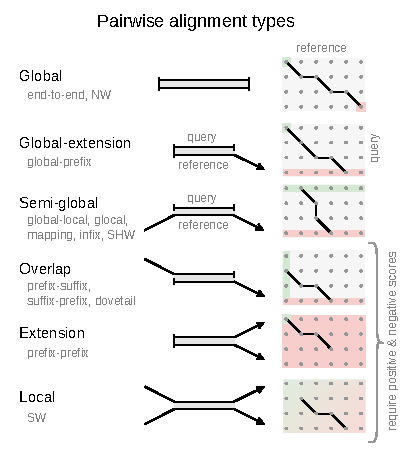
\includegraphics[width=0.5\textwidth]{alignment-types}
	\caption[Alignment types]{Alignment types.}
    \label{fig:alignment-types}
\end{floatingfigure}

% paper-trie; seed-and-extend approach to semi-global alignment
\paragraph{Seed-and-Extend}
Since optimal alignment is often intractable, many aligners use heuristics, most
commonly the \emph{seed-and-extend}
paradigm~\cite{altschul_basic_1990,langmead_fast_2012,li_fast_2009}. In this
approach, alignment initiation sites (\emph{seeds}) are determined, which are
then \emph{extended} to form the \emph{alignments} of the query sequence. The
fundamental issue with this approach, however, is that the seeding and extension
phases are mostly decoupled during alignment. Thus, an algorithm with a provably
optimal extension phase may not result in optimal alignments due to the
selection of a suboptimal seed in the first phase. In cases of high sequence
variability, the seeding phase may even fail to find an appropriate seed from
which to extend.

%%%%%%%%%%%%%%%%%%%%%%%%%%%%%%%%%
%\subsection{Related work}

% Brownie aligner
BrownieAligner, another recent work developed for local alignment of sequences
to {\itshape de Bruijn} graph representations of genomic variation, features an
optimal extension phase using a branch-and-bound-based early cutoff, while
employing a heuristic maximal-exact-match approach for
seeding~\cite{heydari_browniealigner_2018}.
\section{Global alignment}

\subsection{Pangenomes and reference graphs}

The shortest path approach naturally fits more complex references than linear.
In fact, any graph reference (incl. cycles) is fine.

% paper-trie; Accounting for variation
%\para{Accounting for Variation}
First attempts to include variation into the reference data structure were made
by augmenting the local alignment method to consider alternative walks during the
extend step~\cite{schneeberger_simultaneous_2009,palmapper}. This approach has
since been extended from the linear reference case to graph references. To
represent non-reference variation of multiple references during the seeding
stage, HISAT2 uses generalized compressed suffix
arrays~\cite{siren_indexing_2014} to index walks in an augmented reference
sequence, forming a local genome graph~\cite{kim_graphbased_2019}.
VG~\cite{garrison_variation_2018} uses a similar
technique~\cite{siren_indexing_2017} to index variation graphs representing a
population of references.

% paper-trie; The benefit from genome graphs
Historically, a single linear reference sequence has been used to represent the
most common variants in a population. While providing a working abstraction for
most cases, rare or sub-population specific variation is especially hard to
model in this setting, creating a reference allele
bias~\cite{stevenson_sources_2013,brandt_mapping_2015}. Consequently, in the
last few years, the field has shifted first towards using sets of reference
sequences, and more recently to graph data structures (so-called {\em genome
graphs}), to represent many genomes or haplotypes
simultaneously~\cite{dilthey_improved_2015,paten_genome_2017,garrison_variation_2018}.

% Sequencing and variant calling
The analysis and understanding of genetic variation encoded in the genome of an
organism lies at the center of computational biology and medicine. Variation is
usually identified through matching sequences obtained from DNA/RNA-sequencing
back to a reference (genome) sequence in the process of \emph{variant calling},
making the alignment task a core problem in sequence bioinformatics.

% paper:seeds
%\subsection{Problem statement: Alignment as shortest path} \label{SEEDsec:task}
%
In the following, we formalize the task of optimally aligning a read to a
reference graph in terms of finding a shortest path in an \emph{alignment
graph}.

\para{Reference graph}
%
A reference graph $\RG=(\RGV,\RGE)$ encodes a collection of references to be
considered when aligning a read. Its directed edges $\RGE \subseteq \RGV \times
\RGV \times \Sigma$ are labeled by nucleotide letters from $\Sigma =
\{\texttt{A},\texttt{C},\texttt{G},\texttt{T}\}$, hence any walk
$\reference{\pi}$ in $\RG$ spells a string $\sigma(\reference{\pi}) \in
\Sigma^*$.

An alignment of a read $q \in \Sigma^*$ to a reference graph $\RG$ consists of
(i)~a walk $\reference{\pi}$ in $\RG$ and (ii)~a sequence of edits (matches,
substitutions, deletions, and insertions) that transform
$\sigma(\reference{\pi})$ to $q$. An alignment is \emph{optimal} if it minimizes
the sum of edit costs for a given real-valued cost model $\cedits = (\cmatch,
\csubst,\cdel, \cins)$.
%
We assume that edit costs are non-negative---a pre-requisite for the correctness
of \A. Further, we assume that $\cmatch \leq \csubst, \cins, \cdel$---a
prerequisite for the correctness of our heuristic.

We note that our approach naturally works for cyclic reference graphs.

\begin{figure}[t]
	\begin{alignat*}{20}
		(
			&\langle&& u &,& i   &\rangle&,
			&\langle&  v &,& i+1 &\rangle&,
			&&q[i],
			&&\cmatch
		&)&\in \AGE
		&& \quad \text{ if } (u,v,\ell) \in \RGE, \ell = q[i] & \qquad \text{(match)}\\
		%
		(
			&\langle&& u &,& i   &\rangle&,
			&\langle&  v &,& i+1 &\rangle&,
			&&q[i],
			&&\csubst
		&) &\in \AGE
		&& \quad \text{ if } (u,v,\ell) \in \RGE, \ell \neq q[i] & \qquad \text{(substitution)}\\
		%
		(
			&\langle&& u &,& i &\rangle&,
			&\langle&  v &,& i &\rangle&,
			&&\varepsilon,
			&&\cdel
		&) &\in \AGE
		&& \quad \text{ if } (u,v,\ell) \in \RGE & \qquad \text{(deletion)}\\
		%
		(
			&\langle&& u &,& i   &\rangle&,
			&\langle&  u &,& i+1 &\rangle&,
			&&q[i],
			&&\cins
		&) &\in \AGE
		&& \quad & \qquad \text{(insertion)},
	\end{alignat*}
	\caption[Formal definition of alignment graph]{Formal definition of
	alignment graph edges $\AGE \subseteq \AGV[q] \times \AGV[q] \times
	\Sigma_\varepsilon \times \mathbb{R}_{\geq 0}$. Here, $u,v \in \RGV$, $0
	\leq i < |q|$, $\ell \in \Sigma$, and $\varepsilon$ represents the empty
	string, indicating that letter $\ell$ was deleted.}
	\label{SEEDfig:graph-edges}
\end{figure}

\para{Alignment graph}
%
In order to formalize optimal alignment as a shortest path finding problem, we
rely on an \emph{alignment graph} $\AG[q]=(\AGV[q],\AGE[q])$.
%
Its nodes $\AGV[q]$ are \emph{states} of the form $\langle v, i \rangle$, where
$v \in \RGV$ is a node in the reference graph and $i \in \{0, \dots, |q|\}$
corresponds to a position in the read $q$.
%
Its edges $\AGE[q]$ are selected such that any path $\alignment{}{\pi}$ in
$\AG[q]$ from $\langle u, 0 \rangle$ to $\langle v, i \rangle$ corresponds to an
alignment of the first $i$ letters of $q$ to $\RG$.
%
Further, the edges are weighted, which allows us to define an \emph{optimal
alignment} of a read $q \in \Sigma^*$ as a shortest path $\alignment{}{\pi}$ in
$\AG[q]$ from $\langle u, 0 \rangle$ to $\langle v, |q| \rangle$, for any $u, v
\in \RGV$.
%
\cref{SEEDfig:graph-edges} formally defines the edges $\AGE$.

% paper:global
\paragraph{Sequences}
The input sequences $A = \overline{a_0a_1\dots a_i \dots a_{n-1}}$ and $B =
\overline{b_0b_1 \dots b_j \dots b_{m-1}}$ are over an alphabet $\Sigma$ with
$4$ letters. We refer to substrings $\overline{a_i \dots a_{i'-1}}$ as
$\substr Ai{i'}$, to prefixes $\overline{a_0 \dots a_{i-1}}$ as $A_{<i}$, and to
suffixes $\overline{a_i \dots a_{n-1}}$ as $A_{\geq i}$. The \emph{edit
distance} $\ed(A,B)$ is the minimum number of insertions, deletions, and
substitutions of single letters needed to convert $A$ into $B$.

\paragraph{Alignment graph}
Let \emph{state} $\st{i}{j}$ denote the subtask of aligning the prefix $A_{<i}$
to the prefix $B_{<j}$. The \emph{alignment graph} (also called \emph{edit
graph}) $G(V,E)$ is a weighted directed graph with vertices $V = \{\st ij \vert
{0\leq i \leq n}, {0\leq j\leq m}\}$ corresponding to all states, and edges
connecting tasks to subtasks: edge ${\st ij \to \st{i{+}1}{j{+}1}}$ has cost $0$
if ${a_i = b_j}$ (match) and $1$ otherwise (substitution), and edges ${\st ij
\to \st{i{+}1}{j}}$ (deletion) and ${\st ij \to\st{i}{j{+}1}}$ (insertion) have
cost $1$. We denote the root state $\st 00$ by $v_s$ and the target state $\st
nm$ by $v_t$. For brevity we write $f(\st ij)$ as $f \st ij$. The alignment graph is
a natural representation of the alignment problem that provides a base for all
alignment algorithms.

%\section{Task Description: Alignment to Reference Graphs}
\label{TRIEsec:task}

We now describe the task of aligning a query to a reference graph. To this end,
we (i)~introduce the task of optimal alignment on a \emph{reference graph}, and
(iii)~introduce an alternative formulation in terms of an \emph{alignment
graph}, which is the basis for shortest path formulations of the optimal
alignment.
%
\cref{TRIEfig:graph-constructions} summarizes these different graph types.

\para{Reference graph}
We encode the collection of references to which we want to align in a reference
graph, which captures genomic variation that a linear reference cannot
express~\cite{paten_genome_2017,garrison_variation_2018}.
%
We formalize a reference graph as a tuple $\RG=(\RGV,\RGE)$ of nodes $\RGV$ and
directed, labeled edges $\RGE \subseteq \RGV \times \RGV \times \Sigma$, where
the alphabet $\Sigma=\{\texttt{A},\texttt{C},\texttt{G},\texttt{T}\}$ represents
the four different nucleotides.
%
Note that in contrast to sequence graphs~\cite{rautiainen_aligning_2017}, we
label edges instead of nodes.

\para{Path, spelling}
Any path $\pi=(e_1,\dots,e_k) \text { in } \RG$ induces a \emph{spelling}
$\sigma(\pi) \in \Sigma^*$ defined by $\sigma(e_1)\cdots\sigma(e_k)$, where
$\sigma(e_i)$ is the label of edge $e_i$ and $\Sigma^* := \bigcup_{k \in
\mathbb{N}} \Sigma^k$. We note that our approach naturally handles cyclic walks
and does not require cycle unrolling, a feature shared with
\bitparallel~\cite{rautiainen_bitparallel_2019} and
\brownie~\cite{heydari_browniealigner_2018} but missing from
\vg~\cite{garrison_variation_2018}, \pasgal~\cite{jain_accelerating_2019} and
\valigntool~\cite{kavya_sequence_2019}.

\para{Alignment on reference graph}
An \emph{alignment} of \emph{query} $q \in \Sigma^*$ to a reference graph
$\RG=(\RGV,\RGE)$ consists of (i)~a path $\pi \text{ in } \RG$ and (ii)~a
sequence of edit operations (matches, substitutions, insertions, deletions)
transforming $\sigma(\pi)$ to~$q$.

\para{Optimal alignment, edit Distance}
Each edit operation is associated with a real-valued cost ($\cmatch$, $\csubst$,
$\cins$, and $\cdel$, respectively).
An optimal alignment minimizes the total cost of the edit operations converting
$\sigma(\pi)$ to $q$. For optimal alignments, this total cost is equal to the
edit distance between $\sigma(\pi)$ and $q$, \ie, the cheapest sequence of edit
operations transforming $\sigma(\pi)$ into $q$.

We make the (standard) assumption that $0 \leq \cmatch \leq \csubst, \cins,
\cdel$, which will be a prerequisite for the correctness of our approach.

\begin{figure}[t]
	\centering
	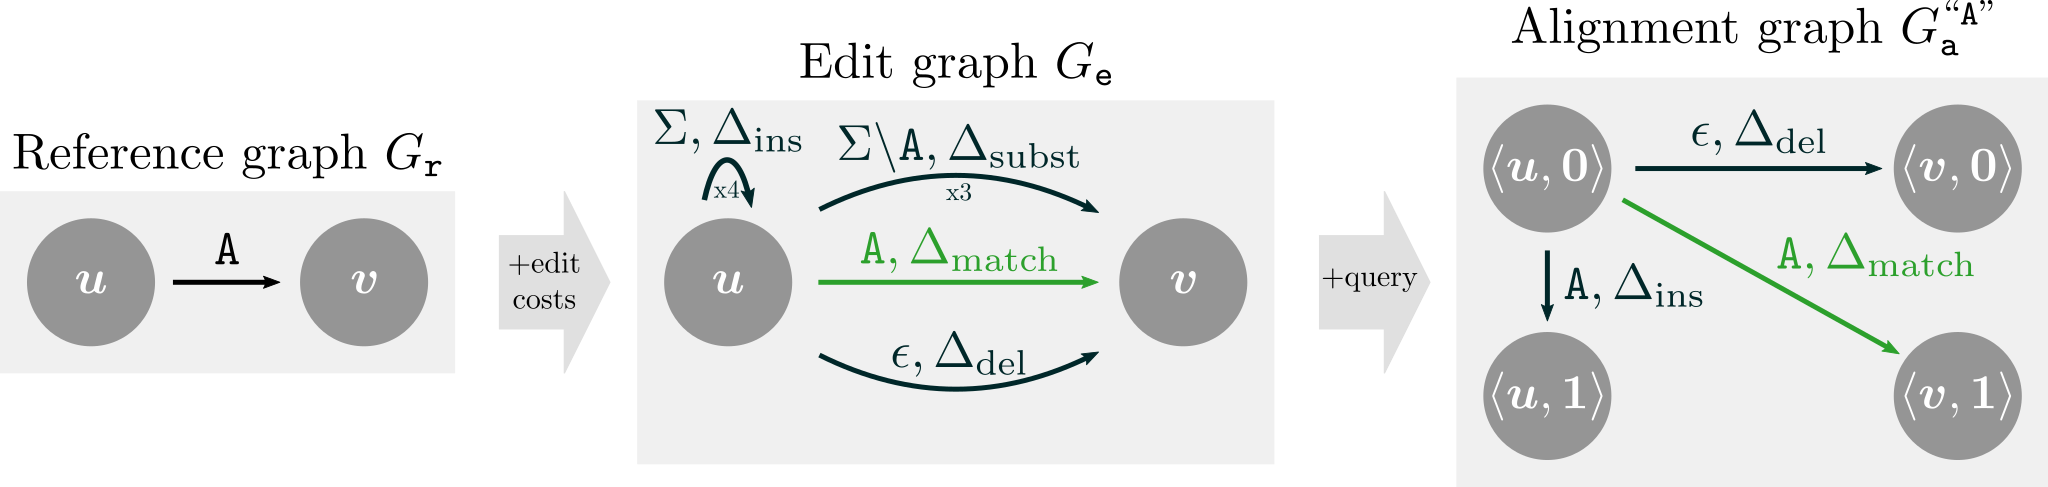
\includegraphics[width=0.8\columnwidth]{edit_graph}
	\caption[Constructing the alignment graph]{Starting from the reference graph
	(left), we can construct the edit graph (middle) and the alignment graph
	$\AG$ for query $q=``\texttt{A}"$ (right). Edges are annotated with labels
	and/or costs, where sets of labels represent multiple edges, one for each
	letter in the set (indicated by $``\text{x}3"$ and $``\text{x}4"$).}
	\label{TRIEfig:graph-constructions}
\end{figure}

% TODO: remove
%\para{Edit graph}
%Instead of representing alignments as pairs of (i)~paths in the reference graph and
%(ii)~sequences of edit operations on these paths, we introduce \emph{edit
%graphs} whose paths intrinsically capture both. This way, we can
%formally define an alignment more conveniently as a path in an edit graph.
%
%Formally, an \emph{edit graph} $\EG:=(\EGV,\EGE)$ has directed, labeled edges
%$\EGE \subseteq \EGV \times \EGV \times \Sigma_\epsilon \times \mathbb{R}_{\geq
%0}$ with associated costs that account for edits. Here, $\Sigma_\epsilon :=
%\Sigma \cup \{\epsilon\}$ extends the alphabet $\Sigma$ by $\epsilon$ to account
%for deleted characters (see \cref{TRIEfig:graph-constructions}).
%%
%The edit and reference graphs consist
%of the same vertices, \ie, $\EGV=\RGV$. However, $\EGE$ contains more edges
%than $\RGE$ to account for edits.
%%
%Concretely, for each edge $(u,v,\ell) \in \RGE$, $\EGE$ contains edges to
%account for (i)~matches, by an edge $(u,v,\ell,\cmatch)$, (ii)~substitutions, by
%edges $(u,v,\ell',\csubst)$ for each $\ell' \in \Sigma \backslash \ell$,
%(iii)~deletions, by an edge $(u,v,\epsilon,\cdel)$, and (iv)~insertions, by
%edges $(u,u,\ell',\cins)$ for each $\ell' \in \Sigma$.
%%
%The spelling $\sigma(\pi) \in \Sigma^*$ of a path $\pi \in \EG$ is defined
%analogously to reference graphs, except that deleted letters (represented by
%$\epsilon$) are ignored. The cost $\cost{\pi}$ of a path $\pi \in \EG$ is the
%sum of all its edge costs.
%
%\para{Alignment on edit Graph}
%An \emph{alignment} of query $q$ to $\RG$ is a path $\pi \text{ in } \EG$
%spelling $q$, \ie, $q=\sigma(\pi)$. An \emph{optimal alignment} is an alignment
%of minimal cost.

\para{Alignment graph}
To find an optimal alignment of $q$ using shortest path finding algorithms, we
must ensure that only paths spelling $q$ are considered. To this end, we
introduce an alternative but equivalent formulation of alignments in terms of an
\emph{alignment graph} $\AG=(\AGV,\AGE)$.

Here, each \emph{state} $\langle v,i \rangle \in \AGV$ consists of a vertex $v \in
\RGV$ and a query position $i \in \{0,\dots,|q|\}$ (equivalent
to~\cite{rautiainen_aligning_2017}). Traversing a state $\langle v,i \rangle \in
\AGV$ represents the alignment of the first $i$ query characters ending at node $v$.
%
In particular, query position $i=0$ indicates that we have not yet matched any
letters from the query.
%
We note that the alignment graph explicitly depends on the query $q$. In
particular, the example alignment graph $\AG[``\texttt{A}"]$ in
~\cref{TRIEfig:graph-constructions} lacks substitution edges from $\AG$, as their
labels ($\texttt{C}$, $\texttt{G}$, $\texttt{T}$) do not match the query
$q=``A"$.

%We construct the alignment graph $\AG$ to guarantee that any walk from a source
%$\langle u,0 \rangle$ to a state $\langle v,i \rangle$ corresponds to an
%alignment of the first $i$ letters of query $q$ to $\RG$.
%As a consequence, there is a one-to-one correspondence between alignments $\edit{\pi}$ of $q$ to
%$\EG$ and paths $\alignment{\pi} \in \AG$ from sources $S:=\RGV \times \{0\}$ to
%targets $T:=\RGV \times \{|q|\}$, with
%$\cost{\reference{\pi}}=\cost{\alignment{\pi}}$. To find the best alignment in
%$\EG$, only paths in $\AG$ (walks without repeating nodes) can be considered,
%since repeating a node in $\AG$ cannot lead to a lower cost ($\cdel \geq 0$) for
%the same state.

%The edges $\AGE \subseteq \AGV \times \AGV \times \Sigma_\epsilon \times
%\mathbb{R}_{\geq 0}$ are built based on the edges in $\EGE$, except that the
%former (i)~keep track of the position in the query $i$, and (ii)~only contain
%empty edges or edges
%whose label matches the next query letter:

\vspace{-1.2em}
{%
\small
\begin{alignat}{10}
	(u,v,\ell,w) &\in \AGE \implies (&\langle u, i \rangle, &\langle v, i+1
		&&\rangle,\ell,w) \in \AGE \quad \text{ for } 0 \leq i < |q| \text{ with }
		q[i]=\ell \label{TRIEeq:alignment-edges-nondeletions} \\
	(u,v,\epsilon,w) &\in\AGE \implies (&\langle u, i \rangle, &\langle v, i
		&&\rangle,\epsilon,w) \in \AGE \quad \text{ for } 0 \leq i < |q| \label{TRIEeq:alignment-edges-deletions}
\end{alignat}
}%

Here, assuming $0$-indexing, $q[i]$ is the next letter to be matched after
matching $i$ letters. Then, \cref{TRIEeq:alignment-edges-nondeletions} represents
matches, substitutions, and insertions (which advance the position in the query
by $1$), while \cref{TRIEeq:alignment-edges-deletions} represents deletions (which do
not advance the position in the query).

\para{Dynamic construction}
As the size of the alignment graph is $\Oh(\lvert \RG \rvert \concat \lvert q
\rvert)$, it is expensive to build it fully for every new query.
Therefore, our implementation constructs the alignment graph $\AG$ on-the-fly:
the outgoing edges of a node are only generated on demand and are freed from
memory after alignment.